\chapter{Organisation}
Dette kapitel omhandler opbygningen af organisationen, hvori teknologien implementeres. I kapitlet undersøges tilrettelæggelse og opgavefordeling i de afdelinger af sundhedssektoren, som påvirkes ved indførelse af Fitbit Flex.

\section{Metode}
Det ønskes at undersøge de organisatoriske forudsætninger samt mulige konsekvenser ved implementering af Fitbit Flex til monitorering af aktivitet i den primære sektor. Undersøgelsen tager udgangspunkt i den modificerede Leavitt organisationsmodel der ses af \autoref{fig:leavittmodel}, for at analysere konsekvenserne af en eventuel ændring i organisationen. Leavitts modificerede organisationsmodel benyttes, da denne tager højde for omgivelsernes påvirkning på teknologi, aktører, opgaver, struktur, disses indbyrdes påvirkning og påvirkning på omgivelserne. 
Teknologi omhandler arbejdsprocesser, procedurer og rutiner, i relation til teknologien.  
Aktører er de ansatte i organisationen, og deres holdninger og ekspertise i relation til organisationens opgaveløsninger. 
Opgaver dækker over de opgavetyper som organisationen forsøger at løse. 
Struktur omhandler formelle mønstre i organisationen, som arbejdsdeling og formalisering.  
Omgivelser er udvalgte interessenter, der er relevante i forhold til de organisatoriske ændringer. 

\begin{figure}[H]
\centering
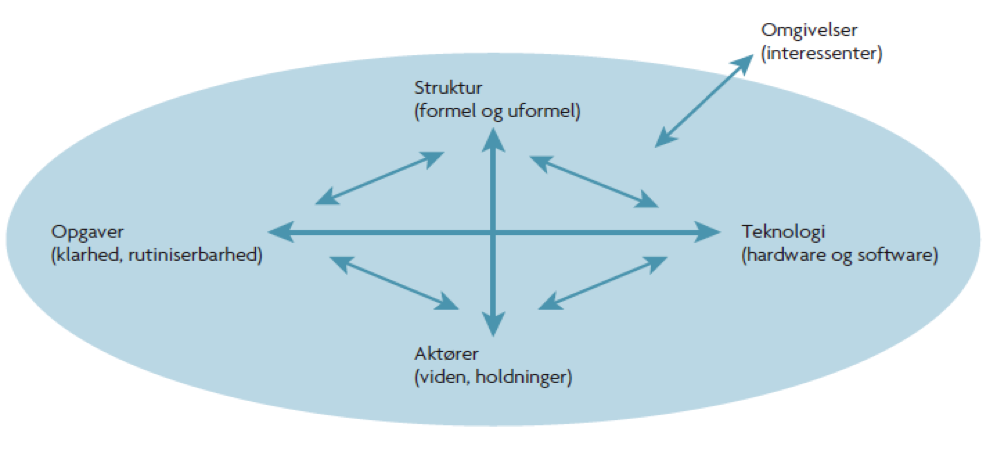
\includegraphics[width=0.9\textwidth]{figures/leavitt}
\caption{Leavitts modificerede organisationsmodel. Pilen mellem de forskellige områder betegner sammenspillet mellem dem. Dertil står omgivelser uden for de andre fire områder, da dette betgener hvem der har interesse for de organisatoriske ændringer der vil forekomme \citep{mtvhaandbog}.}
\label{fig:leavittmodel}
\end{figure}
\noindent
Dette giver anledning til følgende MTV-spørgsmål:

\subsection{MTV-spørgsmål}
\begin{itemize}
\item Hvordan passer Fitbit Flex i den primære sundhedssektor? 
\item Hvilke krav vil implementeringen stille til alment praktiserende læger, og hvem skal stå for en eventuel efteruddannelse? 
% \item Hvilke krav vil implementeringen stille til alment praktiserende læger, og hvad ville omfanget være af en eventuel efteruddannelse?
\item  Hvordan vil patientfordelingen mellem den primære og sekundære sundhedssektor blive påvirket, og hvad vil en ændring i arbejdsfordelingen medføre?
\end{itemize}